\section{Conducting and reporting the search}\label{sec:conducting-and-reporting-the-search}

After the preparations were completed, the next step was to \textbf{perform the searches} in the engines and \textbf{document the results} (search date, search areas, number of results).
The searches were performed from February 6$^{th}$ to February 9$^{th}$, 2023.
Scopus search returned 1414 results;
Web of Science search returned 856 documents.

\begin{samepage}
While conducting the search, the literature was \textbf{tentatively screened for inclusion} based on titles and abstracts of works.
The articles were chosen if they:
    \begin{itemize}
        \item could potentially present a UIDL or a user interface representation
        \item could potentially present an approach to MBUID that might use a UI representation
        \item could potentially present a review of UI representations
        \item could potentially discuss the problem of the expressiveness of UI representations
    \end{itemize}
\end{samepage}
\textbf{The same criteria were also used to search for relevant papers in the following steps.}
The screening was rather broad and not too precise so that \textbf{as much relevant work as possible was identified};
irrelevant literature could be discarded during the later stages of the review.
This stage yielded 133 Scopus documents and 77 Web of Science documents.
After merging the two sets and removing duplicates, 154 documents were left for further consideration.

The second stage of the review eliminated documents unrelated to the subject of the thesis.
At this stage, the decision was also \textbf{based on their introductions and conclusions}.
The process resulted in 47 of them being discarded; in general, due to the focus on issues outside the area of MBUID\@.
Other reasons for exclusion included:
\begin{itemize}
    \item concern about functional/declarative development of UIs
    \item describing methods not focused on generating UIs, but whole applications
    \item relying on, evaluating, or comparing existing UI representations.
    \item lack of a clear description of a UI representation
\end{itemize}

The third stage of the review eliminated additional papers, this time based on \textbf{skimming their full text}.
At this stage, 62 were rejected for the following reasons:
\begin{itemize}
    \item focus on UI or general development
    \item insufficient relation to the thesis problem: interaction modeling, development of an MBUID environment, techniques for UI adaptation
    \item relying on existing work or UI description
    \item lack of a clear definition of a UI description
    \item focus on describing UIs only for specific use cases
    \item lack of access to the full text
\end{itemize}

The last screening step was the exclusion \textbf{based on full-text analysis} of articles.
At this stage, 34 documents were excluded:
\begin{itemize}
    \item papers with an unclear, informal, or incomplete definition of a UI description
    \item papers that further develop existing approaches
    \item papers that use but do not extend an existing UI representation
    \item papers that focus on representing the UI on an abstract level (not the concrete level, according to the CRF)
\end{itemize}

The search results were extended through snowballing, based on the literature from the last screening step.
This process added six additional documents to the results of the review.

\begin{figure}
    \centering
    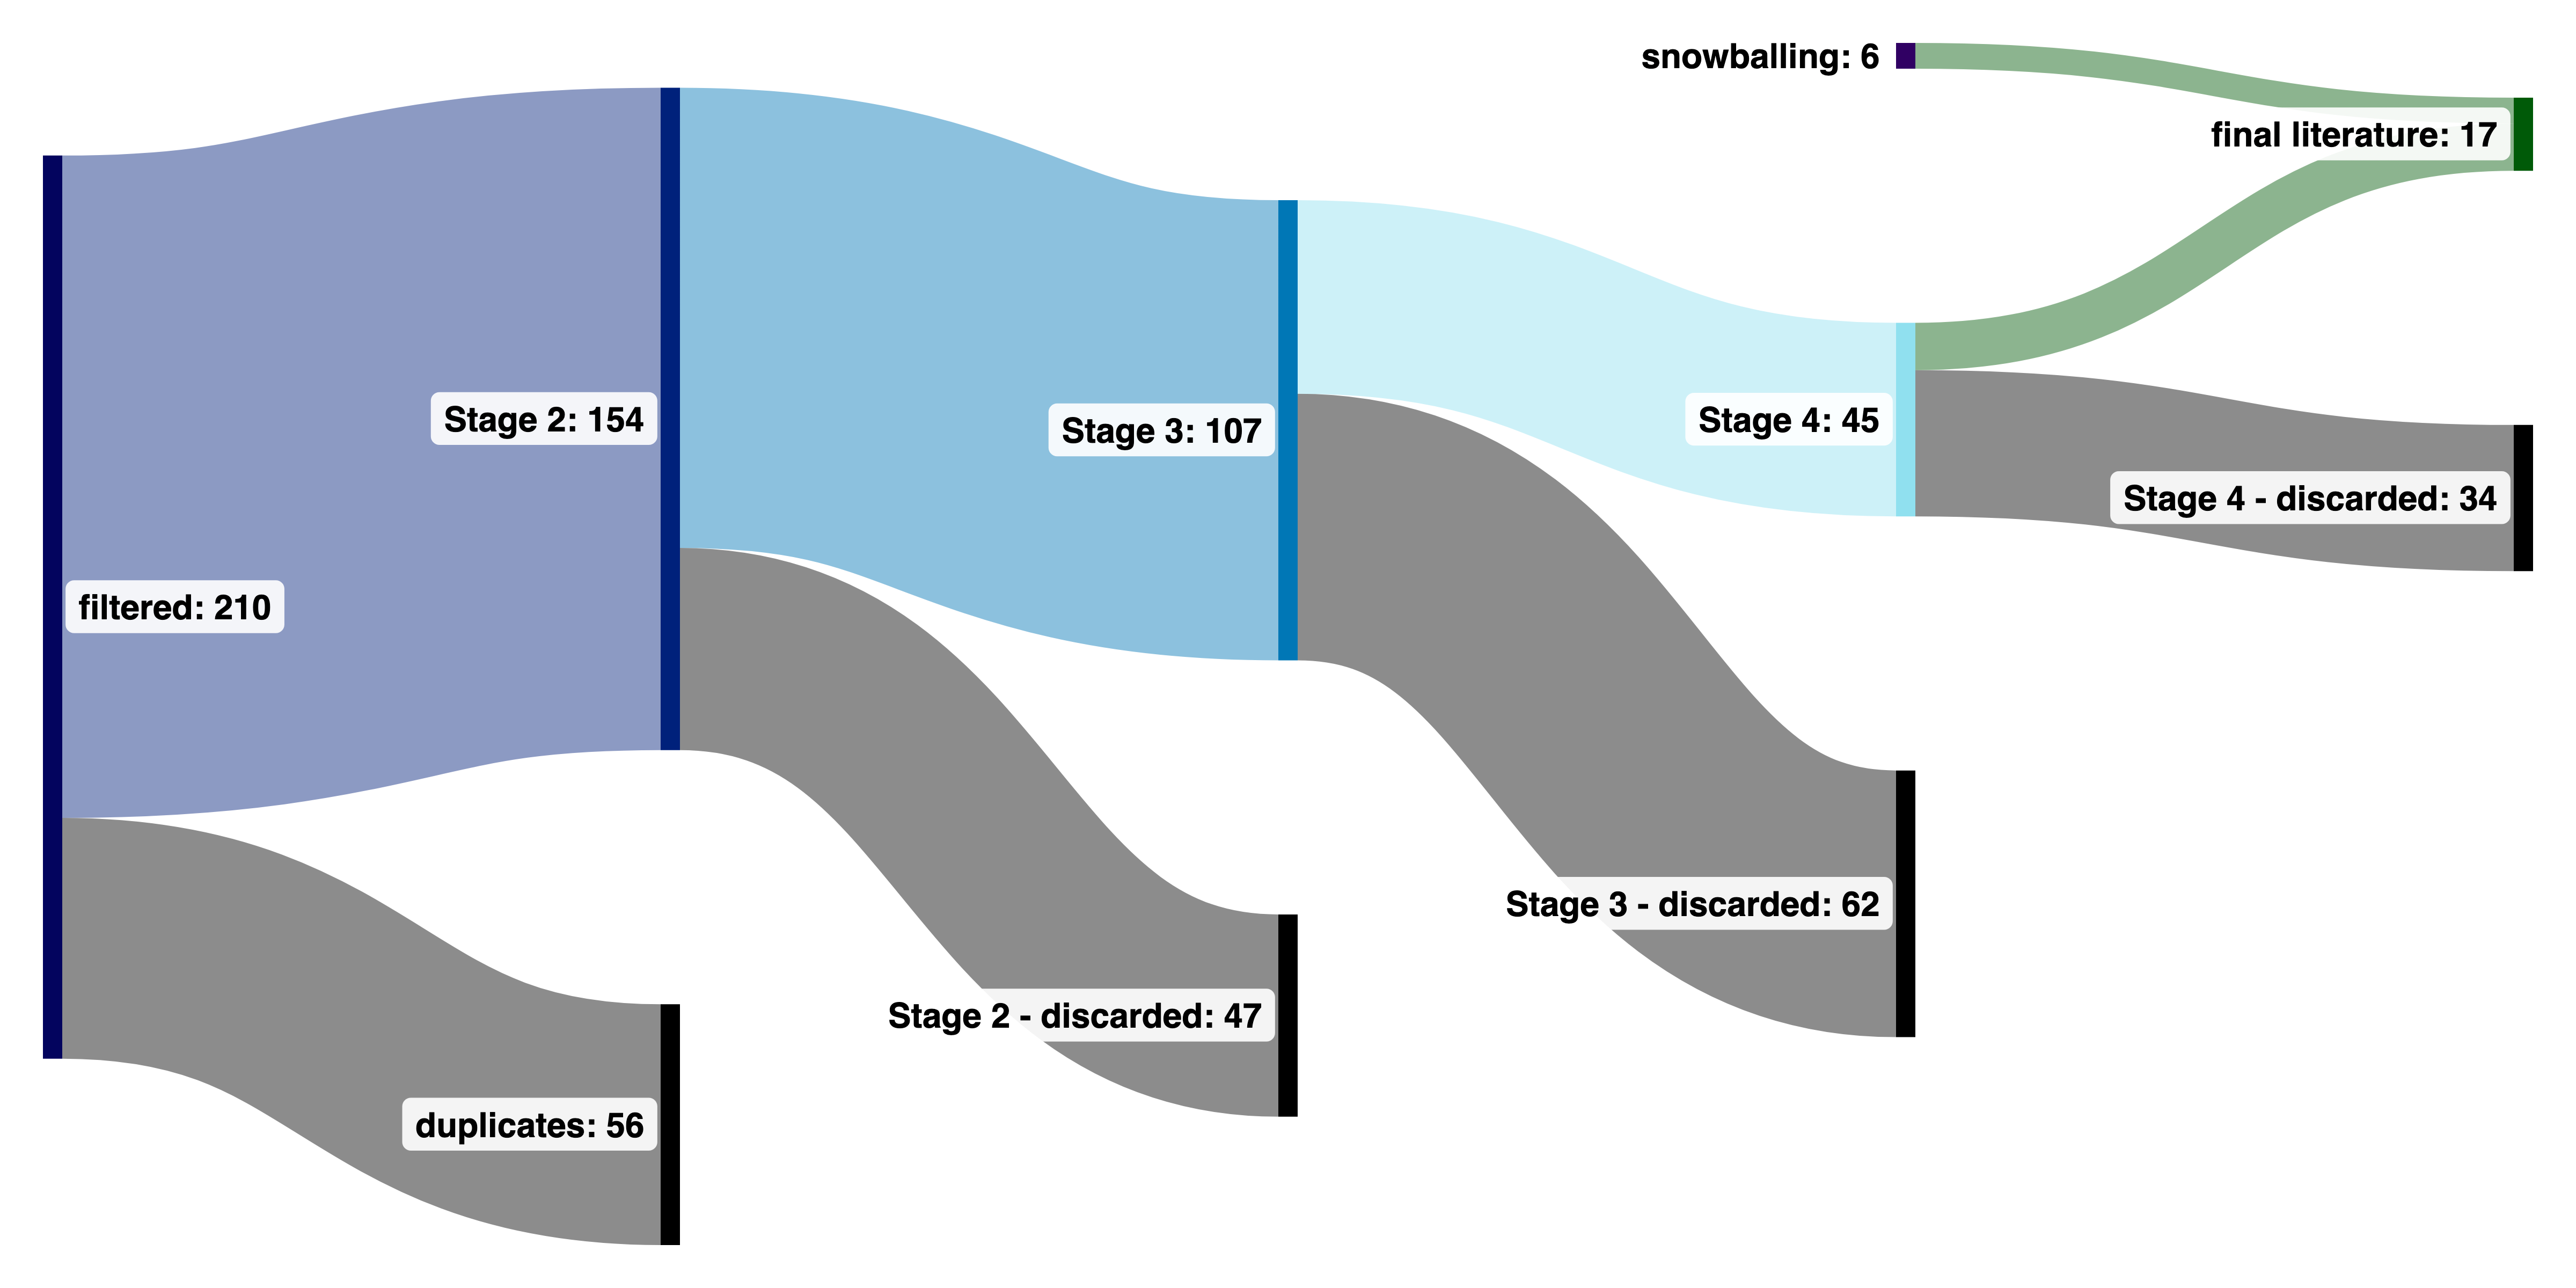
\includegraphics[width=\textwidth]{./2-literature-review/conducting-the-search}
    \caption{Visualization of the subsequent steps of inclusion screening.}
    \label{fig:conducting-the-search-vis}
\end{figure}

In the end, 17 articles were identified during the search.
Figure~\ref{fig:conducting-the-search-vis} summarizes the process.

